% !TEX root =  fission.tex
\pagebreak
\subsection{{\tt MCNPX}}\label{sec:mcnpx}
Version 1.8 of this library was incorporated into the public release of {\tt MCNPX2.7.0}. The authors of this library also maintain private builds of {\tt MCNPX2.7.0} with the most current version of the {\tt LLNL Fission Library}. For users with access to the {\tt MCNPX} source code, upcoming versions of this library can be compiled and linked, see \texttt{src/Recipe\_mcnpx.txt}. Consult the file \texttt{Release\_notes.txt} for comments regarding version compatibility. Currently {\tt MCNPX} provide data cards to activate the fission library (individually for spontaneous, neutron-induced, and photon-induced fission), but do not yet permit changing any of the physics options of the library. 

In addition to adding more neutron multiplicity data and more model options, we made significant modifications to the {\tt MCNPX} treatment of photons, which were then partly carried over into {\tt MCNP6}. The original version of {\tt MCNPX} did not have an analog and discrete treatment for photon emission. Previously photons from fission were included in a total average photonuclear photon count. So it was impossible to have an accurate event-by-event model of photon emission from fission. Our library solved this problem by separating out the photons from the fission process and treating them in a discrete fashion. This took much careful work in cooperation with the {\tt MCNPX} developers. Activating our physics module therefore activates this separate treatment of the fission process as well as provides the features described in this document.

Treatment of fission photons is slightly different in {\tt MCNP6.2}, see {\tt MCNP6.2} User Manual for details.

\subsubsection*{Neutron-induced and spontaneous fission model}

To enable sampling of neutrons and gamma-rays using this fission library set the 6$^{th}$ entry FISM of the PHYS:N card to 5:
\begin{verbatim}
	PHYS:N 5J 5
\end{verbatim}
Note that currently FISM=5 is the only {\tt MCNPX} setting for which gamma-rays are sampled in analog mode for fission reactions. 

Spontaneous fission reactions are activated when definition card SDEF is set to SF:
\begin{verbatim}
	SDEF PAR=SF
\end{verbatim}

In the case of spontaneous fissions, only the isotopes listed in Section~\ref{Limitations of the fission library} have data in the fission library. For other spontaneous fission isotopes, no neutrons, nor gamma-rays are emitted.

\subsubsection*{Photon-induced fission model}

To enable the analog production of photons and neutrons from photofission reactions, the 7$^{th}$ entry FISM of the PHYS:P card should be set to 1:
\begin{verbatim}
        PHYS:P 3J -1 2J 1
\end{verbatim}
When this flag is set, photofission secondaries are sampled only when a photofission event occurs, and are not sampled when other photonuclear reactions occur.

This is different from the default behavior (FISM=0), where photons undergoing photonuclear interactions produce an average number of secondary particles each having a sampled energy/angle though not necessarily from the same photonuclear reaction. The number of secondary particles, as well as their energies and directions are averaged over all possible photonuclear interactions (including photofission). While this default setting is obvisouly not correct microscopically, and we cannot use it to do coincidence counting of photofission neutrons/gammas for instance, it is however correct on average over a large number of interactions.

It is important to note that it is the 4$^{th}$ entry ISPN of the PHYS:P card that controls the analog versus biased nature of the LLNL photofission library collision sampling.

Regarding the data libraries, the physics module needs the ENDF/B-VII photonuclear data library \textit{endf7u}. Lines have to be appended to the file \textit{xsdir} for {\tt MCNPX} to access this photonuclear data library. These lines are also available from the {\tt MCNPX} website. Both \textit{xsdir} and the data library \textit{endf7u} must be in the directory pointed to by the variable DATAPATH.

Photofission is only available for the 39 isotopes listed in Table~\ref{table:photofission isotopes}. Regardless of the option chosen in the $7^{th}$ entry of the PHYS:P card, delayed neutrons and gammas from photofission can be turned on 
and off independently via a different card.

\subsubsection*{Photofission example}

In this example, we will consider a 12 MeV photon beam impinging on a $^{235}$U ball. The photonuclear reaction cross-sections for $^{235}$U are plotted in Fig.~\ref{fig:U-235 photonuclear cross-section}.
%
\begin{figure}[ht]
\begin{center}
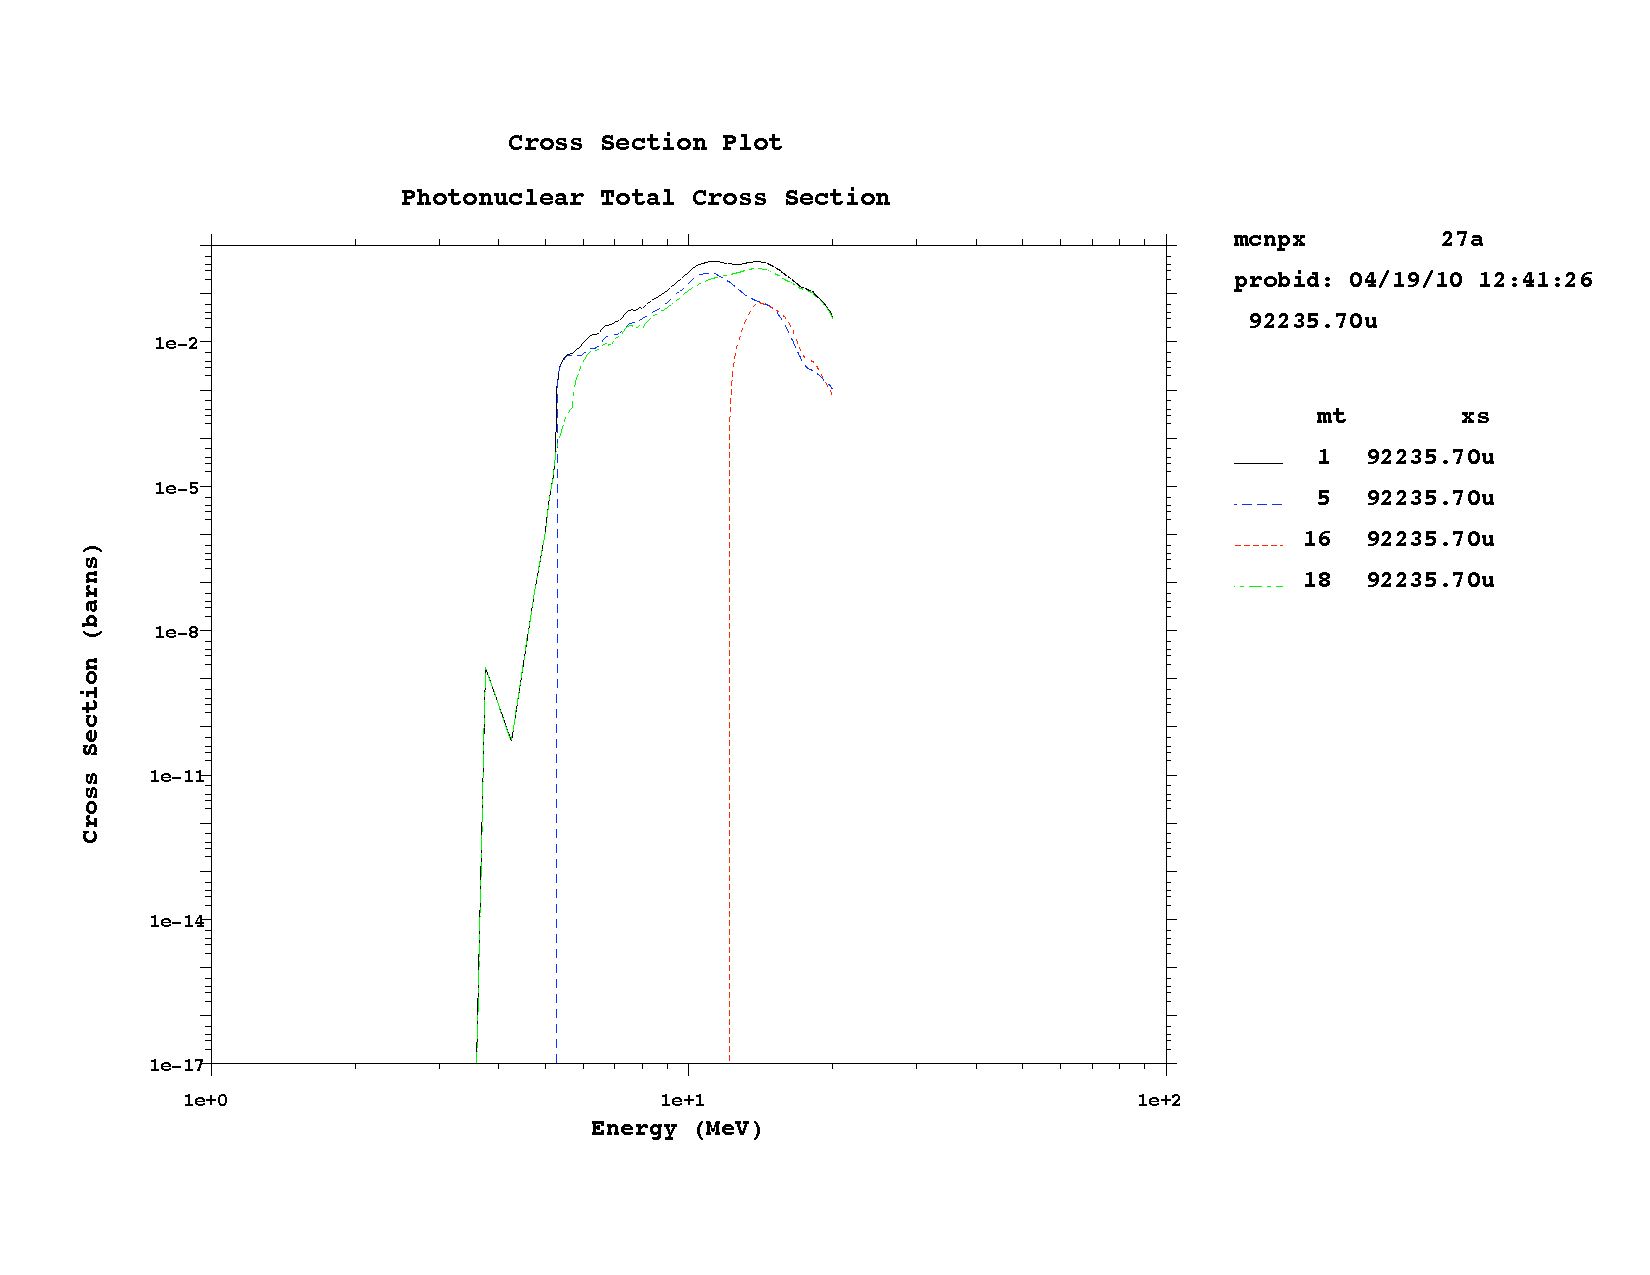
\includegraphics[scale=0.6, angle=0]{eps/92235_photonuclear.pdf}
\end{center}
\caption{Photonuclear cross-sections for $^{235}$U (taken from 92235.70u). Black curve is total, red curve is ($\gamma$,2n), green curve is photofission, blue is all other photonuclear reactions.} 
\label{fig:U-235 photonuclear cross-section}
\end{figure}

The {\tt MCNPX} input deck that describes this example is given below:
{\scriptsize
\begin{verbatim}
12 MeV x-rays into U-235
1 1 -19.0 -1 imp:n=1
2 0 1 imp:n=0

1 so 1.0

mode n p
m1 92235 1 pnlib=.70u
PHYS:P j 1 j -1 2j 1 $ 0=ACE,1=LLNL
sdef par=p erg=12
LCA 7j -2
nps 1000000
f1:n 1
e1 1e-6 199log 12
f11:p 1
e11 1e-3 199log 12
ft11 tag 3
fu11 -1 0.00004 92000.00003 92235.00005 92000.00005 92235.00018 1e10
\end{verbatim}}

To switch from the default ACE {\tt MCNPX} model to the LLNL photofission library, the $7^{th}$ entry of the PHYS:P is set to 1 in the input deck. Note that the $4^{th}$ entry of the PHYS:P card is set to -1 to turn on analog photonuclear particle production. We are interested here in the spectrum of prompt photofission gamma-rays emitted by $^{235}$U. Figure~\ref{fig:energy spectrum of the photofission gamma-rays from a 12 MeV gamma-ray beam impinging on 235U} shows the energy distribution of the photofission gamma-rays for different {\tt MCNPX} settings.

\begin{figure}[ht]
\begin{center}
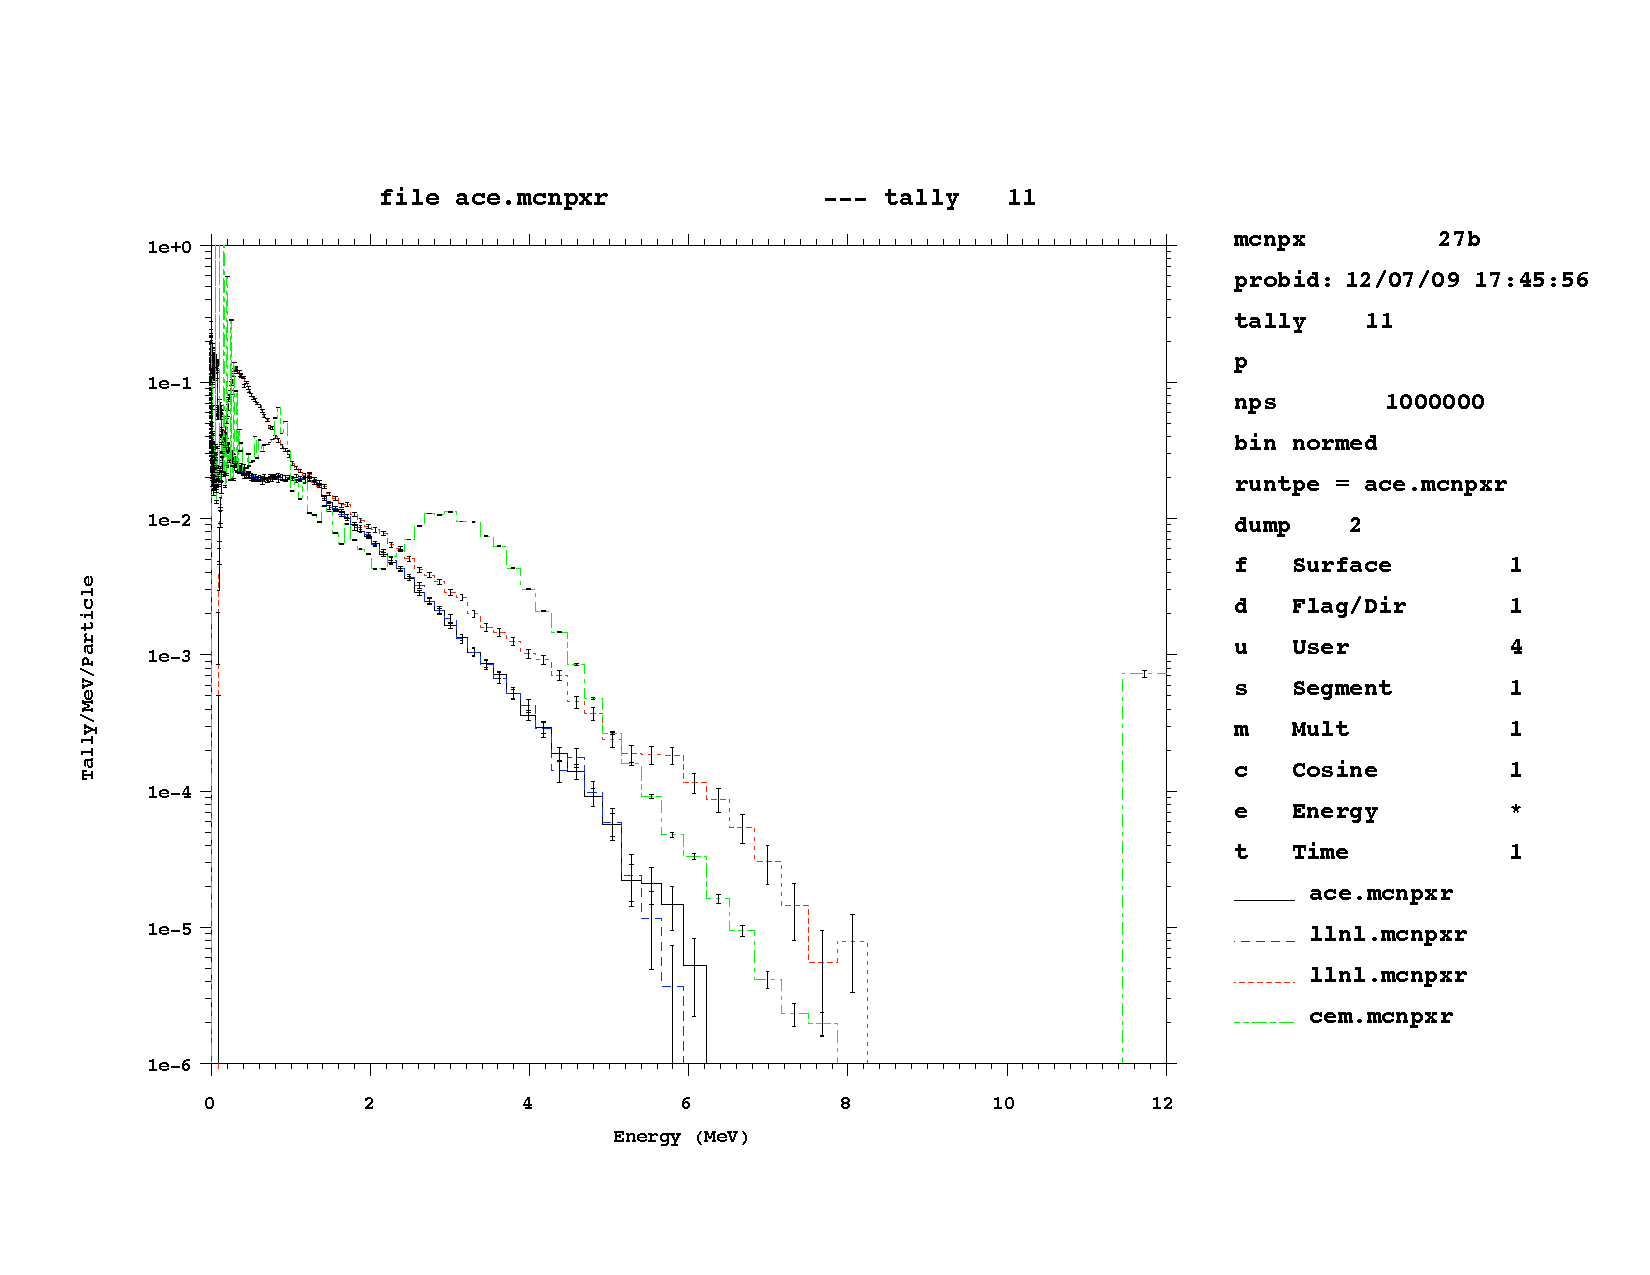
\includegraphics[width=\textwidth]{eps/PhotofissionGammaSpectrum.pdf}
\end{center}
\caption{Energy spectrum of the photofission gamma-rays from a 12 MeV gamma-ray beam impinging on $^{235}$U. The black, blue \& red, and green curves were generated by {\tt MCNPX} simulations with the ACE, LLNL, and CEM models, respectively.}
\label{fig:energy spectrum of the photofission gamma-rays from a 12 MeV gamma-ray
beam impinging on 235U}
\end{figure}

The black curve was generated from a  simulation with the ACE model, it shows the spectrum of all gamma-rays produced 
by photonuclear reactions with the ACE model. The default {\tt MCNPX} ACE model produces prompt photofission 
neutrons but does not produce any prompt photofission gamma-rays, because there is no such data available in the 
photonuclear data libraries ENDF/B-VII. 

The blue and red curves were generated from a simulation where the LLNL photofission library was turned on. The red curve is the spectrum of gamma-rays produced by photofission, while the blue one corresponds to gamma-rays produced by all other photonuclear reactions.

Finally, a last simulation was performed with the much slower CEM model, and the green curve shows the gamma-ray spectrum of all photonuclear reactions with this model.

\subsection{{\tt MCNP6}}\label{sec:mcnp}

Version 1.8 of this library was incorporated into the public release of {\tt MCNP6}. Version 2.0 is now incorporated into {\tt MCNP6.2}. For users with access to the {\tt MCNP6} source code, upcoming versions of this library can be compiled and linked, see \texttt{src/Recipe\_mcnpx.txt}. Consult the file \texttt{Release\_notes.txt} for comments regarding version compatibility.
Currently {\tt MCNP6} provide data cards to activate the fission library (individually for spontaneous, neutron-induced, and photon-induced fission), but do not yet permit changing any of the physics options of the library. 

In {\tt MCNP6.2}, treatment of fission photons is slightly different from what it is in {\tt MCNPX2.7.0}. See {\tt MCNP6.2} User Manual for details.

\subsubsection*{Neutron-induced and spontaneous fission model}

To enable sampling of neutrons and gamma-rays using this fission library set the {\tt METHOD} keyword on the FMULT card
to 5:
\begin{verbatim}
	FMULT zaid METHOD=5
\end{verbatim}
The LLNL fission model is the only way in {\tt MCNP6.2} to produce prompt fission photons. When the LLNL fission multiplicity package is selected (METHOD=5), both the prompt neutrons and the prompt fission photons are fully correlated with the fission event and have multiplicities.

Furthermore, when spontaneous fission reactions are activated, i.e.,
\begin{verbatim}
	SDEF PAR=SF
\end{verbatim}
the LLNL model is the only {\tt MCNP6} method emitting prompt photons for spontaneous fissions. In the case of spontaneous fissions, only the isotopes listed in Section~\ref{Limitations of the fission library} have data in the fission library. For other spontaneous fission isotopes, no neutrons, nor gamma-rays are emitted. Spontaneous fission photons are neglected in the {\tt MCNP6} default FMULT spontaneous fission source.

Delayed fission gammas are independent of the fission model and are controlled by the ACT card.

\subsubsection*{Photon-induced fission model}

When METHOD 5 is selected on the FMULT card and photofission is also turned on (ISPN$\ne$0 and FISM=1 on the PHYS:P card):
\begin{verbatim}
        PHYS:P 3J -1 2J 1
\end{verbatim}
prompt photofission gammas are generated with appropriate photofission neutron correlation and multiplicities. The same remarks as the ones in Sec.~\ref{sec:mcnpx} for the photon-induced fission model, apply here as well.

